\documentclass[11pt]{article}
\usepackage[margin=1in]{geometry}
\usepackage[utf8]{inputenc}
\usepackage[T1]{fontenc}
\usepackage{lmodern}
\usepackage{microtype}
\usepackage{amsmath,amssymb}
\usepackage{booktabs}
\usepackage{graphicx}
\usepackage{xcolor}
\usepackage[numbers,sort&compress]{natbib}
\usepackage[hidelinks]{hyperref}
\usepackage[capitalise,noabbrev]{cleveref}

% Every result number is a macro written by figures/make_figures.py from the
% measured JSON in bench/results.  A key that was not measured renders as a
% visible red PENDING marker instead of silently disappearing.
\newcommand{\res}[1]{\ifcsname res:#1\endcsname\csname res:#1\endcsname\else\textcolor{red}{\textbf{PENDING}}\fi}
\newcommand{\pending}[1]{\textcolor{red}{\textbf{PENDING:}}~#1}
\InputIfFileExists{generated/results.tex}{}{}

\title{Mid-Decode Model Migration Under a Per-App Memory Limit:\\
Moving a Generation to a Smaller Model Without Holding Both}
\author{NagaYu\thanks{Code, mappers and raw measurements: \url{https://github.com/NagaYu/molt}.
\ Draft generated \today; device results pending (see \cref{sec:limits}).}}
\date{}

\begin{document}
\maketitle

\begin{abstract}
\noindent\textbf{Prior work first.}
Closed-form ridge maps between the KV caches of different-size models in one family were introduced by Heo et al.~\citep{heo2026crossmodel}.
They apply them at the \emph{prefill hand-off point}.
DroidSpeak~\citep{liu2024droidspeak} shares KV caches between models that have the same architecture and are fine-tuned from the same base.
This paper adds no new mapping and claims nothing about mapping quality.
Its scope is limited to three conditions that this prior work does not address:
the switch happens \emph{mid-decode}, between two tokens of one generation;
it happens \emph{under memory exhaustion}, triggered by the app's distance to its own per-process limit;
and the two models are \emph{never resident together}.

We implement this setting in MLX on Apple silicon and test it against an external jetsam emulator.
We compare it with restart, always-small, re-prefill, and the closed-form ridge map of~\citep{heo2026crossmodel} applied mid-decode.
That last baseline is reproduced to the letter and runs in the hand-off shape, with both models loaded.
On two Qwen2.5 pairs (1.5B$\to$0.5B and 3B$\to$1.5B, 4-bit), a switch that loads the receiver before releasing the sender is killed whenever the app has less spare memory than it needs.
Every release-first switch survives.
But the transferred cache loses the prompt's specifics.
On a needle task with a 3B$\to$1.5B switch just before the answer, the mapped cache answers \res{q.3b-15b.D.needle} with our additions and \res{q.3b-15b.C.needle} without, against \res{q.3b-15b.A2.needle} when the small model simply re-reads the transcript.
At $\sim$2\,100 tokens the transfer resumes \res{qp.3b-15b.D.A2.longneedle.resume}\,s sooner but answers \res{q.3b-15b.D.longneedle} against \res{q.3b-15b.A2.longneedle}.
In the setting we claim, KV transfer is not the right way to switch, and we state where our own hypothesis fails.
iPhone measurements, energy on device, and human ratings are \pending{not yet collected}.
\end{abstract}

\section{Scope and prior work}\label{sec:intro}

\paragraph{What is not ours.}
Mapping one model's KV cache into another model's geometry is prior work.
Heo et al.~\citep{heo2026crossmodel} fit, for every target layer and KV head, separate key and value maps in closed form by ridge regression ($\lambda=0.01$).
The input is the concatenated KV heads of the top-$k$ source layers, ranked by single-source $R^2$.
Keys have RoPE~\citep{su2021roformer} removed before the map and re-applied after it.
The transfer happens at the \emph{prefill hand-off point}: the receiver gets the sender's prefix cache and decodes from there.
Their main results are small-to-large over matched KV geometry.
Large-to-small is reported only on HellaSwag, where one pair keeps 37\% of standalone accuracy.
DroidSpeak~\citep{liu2024droidspeak} reuses KV caches between models that share an architecture and a foundation model.
It recomputes selected layers and reuses the rest, at prefill time.
Re-reading a transcript with a new model (re-prefill) is a standard alternative, and we treat it as a baseline.
Keeping the first tokens because attention concentrates on them follows StreamingLLM~\citep{xiao2023streamingllm}.

\paragraph{What this paper claims, and only this.}
We study one situation.
An on-device app is in the middle of generating an answer with a model that nearly fills the app's memory budget.
Then something else in the app needs memory.
On iOS the app is killed once it crosses its per-process limit~\citep{apple_jetsam}.
The goal is to continue \emph{the same sentence} with a smaller model, with no retracted tokens and no termination.
The contribution is restricted to three conditions:
\begin{enumerate}
\item \textbf{Mid-decode.} The switch happens between two tokens of one generation. The receiver takes the sender's cache for every token fed so far and itself feeds the token already shown to the user.
\item \textbf{Under memory exhaustion.} The switch is triggered by the app's headroom to its own limit (\texttt{os\_proc\_available\_memory}~\citep{apple_os_proc_available_memory}), polled before every token, before the limit is crossed.
\item \textbf{Non-co-resident.} Sender and receiver weights are never resident together. We show what this requires on MLX~\citep{mlx2023} and test that the kernel-tracked peak footprint stays under the cap.
\end{enumerate}
Nothing else in this paper is claimed as new.
That includes the mapping, its fitting procedure, RoPE handling, re-prefill and sink tokens.

\paragraph{The question that decides whether there is a claim at all.}
If the simple method is enough in this setting, molt has nothing to claim.
The simple method is the closed-form map of~\citep{heo2026crossmodel} applied at the token boundary.
We therefore reproduce it without shortcuts (condition C) and measure where it is and is not enough.
\Cref{sec:failures} states plainly where our own hypothesis fails.

\section{The setting}\label{sec:problem}

\paragraph{The limit an app actually faces.}
Apple documents \texttt{os\_proc\_available\_memory()} as ``the current memory limit minus the memory footprint of your app''.
It returns 0 once the limit is exceeded.
The limit can change during the app's life cycle, and the value is advisory and should not be cached~\citep{apple_os_proc_available_memory}.
A jetsam event report records the reason for a termination.
\texttt{per-process-limit} means the app crossed the limit imposed on all apps; \texttt{vm-pageshortage} means system-wide pressure~\citep{apple_jetsam}.
The UIKit memory warning~\citep{apple_memwarning} and the dispatch memory-pressure source~\citep{apple_pressure_source} report \emph{system} memory pressure.
We found no documentation that promises either one fires before a \texttt{per-process-limit} termination.
Some devices honour a larger limit under the \texttt{increased-memory-limit} entitlement~\citep{apple_increased_limit}.
The quantity the limit is checked against is the physical footprint.
On Apple silicon, MLX tensors sit in Metal buffers that the resident set size barely counts.
We measured a 1\,GiB MLX array moving RSS by $\approx$0\,MiB and the footprint by $\approx$1\,GiB.
Every memory number in this paper is therefore phys\_footprint, never RSS.

\paragraph{The event.}
A generation runs on model $S$, whose footprint leaves headroom $h$ under the limit.
At token $n_p$, the app's other work starts to need $B$ more memory, arriving in chunks of 64\,MiB per token.
$B$ exceeds $h$, so $S$ cannot stay, while the smaller model $T$ plus $B$ fits.
A condition survives if its footprint never exceeds the limit.
A co-resident switch needs about $T$'s weights plus the mapper in spare memory at the moment it starts.
A non-co-resident switch needs only the KV caches and the mapper.
The interesting band is
\[
  \underbrace{\text{chunk} + \text{margin}}_{\text{ordered needs}} \;\le\; h \;<\; \underbrace{w_T + w_{\text{map}} + \text{margin}}_{\text{co-resident needs}},
\]
where one schedule survives and the other cannot.
\Cref{sec:results-memory} measures whether the band exists and how wide it is for real tiers.

\section{Method}\label{sec:method}

\subsection{The mapping (prior work, condition C)}\label{sec:heo}
We reproduce the recipe of~\citep{heo2026crossmodel} as written.
\begin{itemize}
\item \emph{Features.} Per source layer, all KV heads are flattened. Keys have the source RoPE removed; values are used as is.
\item \emph{Targets.} The destination's own keys (RoPE removed) and values, per layer and head.
\item \emph{Regression.} Centred ridge with $\lambda=0.01$ and bias $b=\bar y-\bar xW$. Covariance is accumulated in float32 and solved in float64.
\item \emph{Data.} 500 FineWeb-Edu~\citep{penedo2024fineweb} sequences of 1\,024 tokens, sub-sampled with stride 4.
\item \emph{Source selection.} For each destination layer, the top-$k$ source layers are kept by a fixed ranking: head-averaged single-source $R^2$, averaged over K and V.
\end{itemize}
Keys are re-rotated with the destination RoPE at the same absolute positions.

We had to make two interpretations, and we state both.
(i) The text writes $X^\top X+\lambda I$ without saying whether $X^\top X$ is normalised.
On $\sim$128\,K rows an unnormalised Gram matrix would make $\lambda=0.01$ a no-op, and their reported collapse at $\lambda=1$ could not happen.
We therefore read $X^\top X$ as the centred covariance and also sweep $\lambda$ (\cref{tab:lambda}).
(ii) Heo et al.\ choose $k$ by downstream accuracy.
We choose $k$ by held-out prefix-KV negative log-likelihood (NLL), measured on documents disjoint from both the calibration and the evaluation splits.

Implementation checks in \texttt{fit.selftest} and \texttt{migrate.selftest}:
a planted linear map is recovered to $R^2=1$;
the $R^2$ computed from sufficient statistics equals the $R^2$ of actually applying the fitted mapper to within $10^{-7}$;
and with an identity mapper, transplanting reproduces a native re-prefill to within $1.4\times10^{-6}$.

\subsection{Mid-decode transplant}\label{sec:transplant}
The decode loop keeps one invariant: the cache holds KV for exactly the tokens fed so far, and \texttt{pending} is the token already shown to the user but not yet fed.
At a switch the receiver gets the mapped cache and feeds \texttt{pending} itself, so no shown token is retracted.
Molt adds two optional \emph{anchors}, which we treat as engineering choices and not as contributions.
\begin{itemize}
\item The first $s$ positions are replaced by the receiver's native KV. This is exact, because causal positions depend only on earlier tokens; it follows the sink observation of~\citep{xiao2023streamingllm}.
\item The last $t$ positions are re-fed natively over the mapped history.
\end{itemize}
Setting $t=\text{all}$ gives re-prefill (condition A$'$).
$s$ and $t\le 32$ are chosen on held-out text only.

\subsection{The memory order (the claim)}\label{sec:order}
Releasing a model on MLX is not one call.
We measured three facts (\cref{app:mlx}).
(1) After \texttt{del}, buffers stay in MLX's allocator cache and are not reused for arrays of other sizes.
(2) \texttt{mx.clear\_cache()} right after \texttt{del} can free nothing, because a buffer returns to the cache only after the GPU has finished the last command buffer that used it.
(3) After synchronising and clearing, the OS still reclaims the memory asynchronously, in about $10^2$\,ms.
The \emph{ordered} schedule therefore runs as follows:
\begin{enumerate}
\item snapshot the source KV;
\item drop the source weights, synchronise, clear, and poll phys\_footprint until it has fallen by 90\% of the source weight bytes;
\item load the mapper and map;
\item drop the mapper and source KV the same way;
\item load the receiver;
\item apply the anchors and resume.
\end{enumerate}
\Cref{tab:schedules} lists the three alternatives we measure against it.
\emph{colocated} is the prefill hand-off shape.
\emph{del-only} is the natural ``drop it, then load''.
\emph{clear-no-wait} is the call a developer would write.

\paragraph{The trigger.}
Before every token the loop reads the headroom.
On iOS that is the return value of \texttt{os\_proc\_available\_memory()}; on the Mac it is $\text{cap}-\text{phys\_footprint}$.
It migrates when the headroom falls below what \emph{the chosen schedule} needs plus the next demand chunk.
Each schedule thus gets its own best trigger, and a co-resident schedule is never killed merely for reacting late.

\section{Experimental setup}\label{sec:setup}

\paragraph{Models.}
We use Qwen2.5 Instruct~\citep{qwen25} in the 4-bit MLX builds an app would ship.
The pairs, large to small (the direction memory pressure forces), are 3B$\to$1.5B (matched KV geometry: 2 KV heads, $d_h=128$) and 1.5B$\to$0.5B (mismatched: $d_h$ 128$\to$64).
Mappers are fitted on these exact 4-bit weights.
All three sizes share one tokenizer, which we checked by vocabulary hash.
Decoding is greedy, so conditions differ only in what the switch did.

\paragraph{Conditions.}
All conditions run on one machine.
Each run is a separate process, so no condition inherits another's allocator state.
\begin{itemize}
\item \textbf{A} restart: discard the generation and start over on the small model.
\item \textbf{A$'$} re-prefill: release, load small, and re-read the prompt plus everything shown so far. This baseline is added because it is the obvious alternative; it is not one of the four named in the brief.
\item \textbf{B} always small.
\item \textbf{C} the closed-form map of~\citep{heo2026crossmodel} applied at the token boundary, with the selected $k^*$, in hand-off shape (colocated) and without anchors.
\item \textbf{D} molt: the same mapper, the ordered schedule and the held-out-selected anchors.
\end{itemize}
Ablations change one factor each:
C$+$ordered isolates the schedule, D$+$colocated the anchors, D with the depth-linear mapper the mapper.
D with del-only and D with clear-no-wait test the naive freeing variants.

\paragraph{Jetsam emulation.}
A separate C process polls the worker's \texttt{proc\_pid\_rusage} at about 1\,kHz.
It records the instantaneous phys\_footprint and the kernel ledger's lifetime maximum (\texttt{ri\_lifetime\_max\_phys\_footprint}), and sends \texttt{SIGKILL} the moment either exceeds the cap.
The lifetime maximum cannot miss a spike between samples.
Phase labels written by the worker attribute every sample to a phase.

\paragraph{Experiments.}
\emph{I (intrinsic)}: teacher-forced NLL of 128 held-out tokens after the switch, on the FineWeb-Edu evaluation split, at boundary positions $P\in\{32,128,256,512,768\}$.
\emph{Q (quality)}: no cap, with the switch at a fixed token per item.
The suite has GSM8K~\citep{cobbe2021gsm8k} (switch at token 32, mid-reasoning), a needle task with 14 similar records (switch right before the answer value), and open-ended explanations (switch at token 48).
\emph{M (memory)}: a cap of $S+h$, where $S$ is the measured footprint of the big model decoding, swept over $h$; demand arrives as in \cref{sec:problem}.

\paragraph{Metrics.}
\begin{itemize}
\item \textbf{Survival}: the run was not killed.
\item \textbf{Lost tokens}: tokens shown and then retracted.
\item \textbf{Visible seam}: the jump in judge NLL across the boundary, $\overline{\text{NLL}}[b,b{+}16)-\overline{\text{NLL}}[b{-}16,b)$, reported relative to A$'$; and human ratings, which are pending.
\item \textbf{Continuation quality}: task accuracy, with a killed run scoring 0 and never dropped, plus judge top-1 agreement after the boundary. The judge is the pair's large model.
\item \textbf{Time to resume}: from trigger to the next shown token. For A, the time until new content appears.
\item \textbf{Peak footprint during migration}: kernel lifetime maximum.
\item \textbf{Energy}: CPU energy per process (\texttt{ri\_energy\_nj}) and GPU energy system-wide from IOReport minus an idle baseline (\cref{app:energy}).
\end{itemize}
Throughput is recorded but is not a primary metric.
Every aggregate carries a 95\% bootstrap interval, paired by item where two conditions are compared.

\paragraph{Platform.}
Reported per run in the result files: \res{env.machine}.
Other users' processes were running during the measurements and swap was nearly full (\cref{sec:limits}).
Timings are reported but should be read with that in mind; footprint and survival are not affected.

\section{Results}\label{sec:results}
\begin{table}[t]\centering\caption{Every fitted mapper. Held-out = documents disjoint from calibration and evaluation.}\label{tab:fit}\textcolor{red}{\textbf{PENDING}}\end{table}

\begin{table}[t]\centering\caption{Ridge $\lambda$ sweep at the selected $k^*$ (centred-covariance reading).}\label{tab:lambda}\textcolor{red}{\textbf{PENDING}}\end{table}

\begin{table}[t]\centering\caption{Experiment Q. Accuracy counts every item; jump = judge-NLL jump at the switch (16 tokens each side).}\label{tab:quality}\textcolor{red}{\textbf{PENDING}}\end{table}

\begin{table}[t]\centering\caption{Experiment M: every cell. Peak = kernel lifetime-max phys\_footprint (MiB).}\label{tab:memory}\textcolor{red}{\textbf{PENDING}}\end{table}


\subsection{The prior mapping, reproduced}\label{sec:results-fit}
\Cref{fig:ksweep,tab:fit} cover every fitted mapper.
\pending{measurements for this subsection.}


\begin{figure}[t]\centering
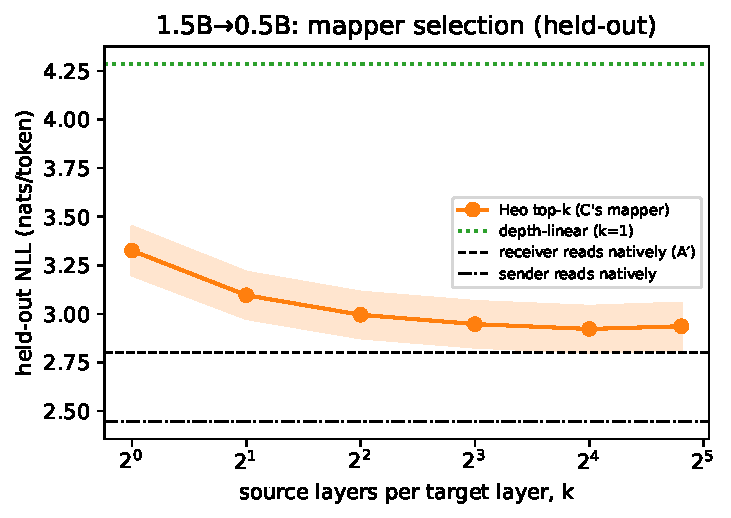
\includegraphics[width=\linewidth]{../figures/paper/fit_ksweep.pdf}
\caption{Held-out prefix-KV NLL against the number of source layers $k$ used by the closed-form mapper of~\citep{heo2026crossmodel}, with 95\% CIs.
Dashed: the receiver reading the same prefix natively (what re-prefill achieves). Dash-dot: the sender reading it natively.}
\label{fig:ksweep}
\end{figure}

\subsection{Transfer cost against switch position}\label{sec:results-intrinsic}
\pending{measurements for this subsection.}


\begin{figure}[t]\centering
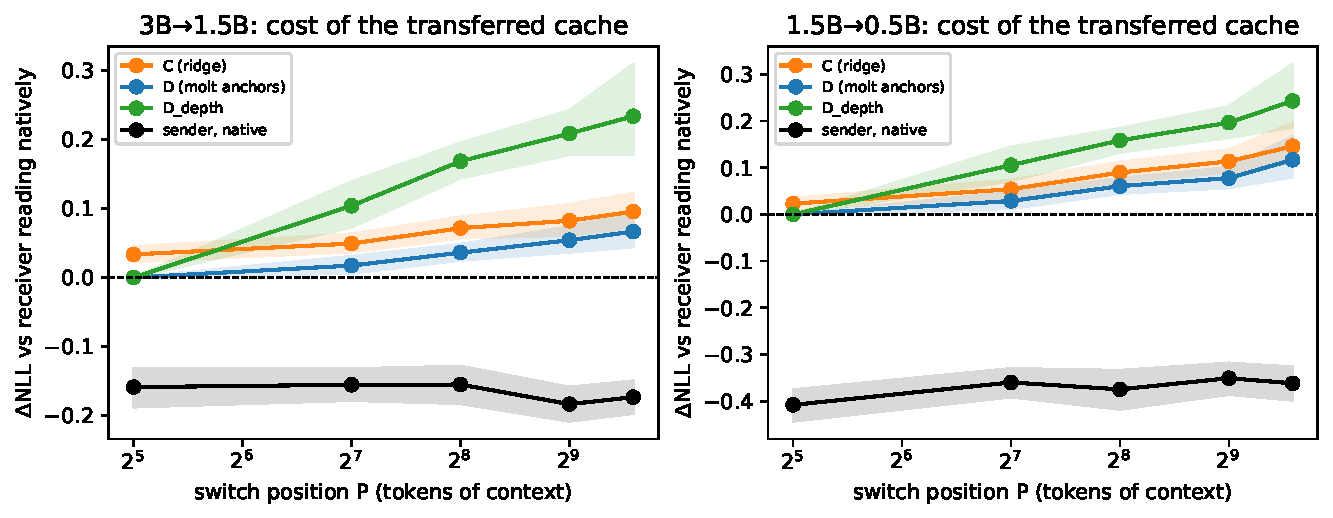
\includegraphics[width=\linewidth]{../figures/paper/intrinsic_context.pdf}
\caption{Experiment I. Extra NLL of the receiver decoding from a transferred cache, relative to reading the same text natively, as a function of how much context precedes the switch. Bands are paired 95\% CIs over evaluation documents.}
\label{fig:intrinsic}
\end{figure}

\subsection{Quality when the switch lands mid-decode}\label{sec:results-quality}
\pending{measurements for this subsection.}


\begin{figure}[t]\centering

\includegraphics[width=\linewidth]{../figures/paper/quality.pdf}
\caption{Experiment Q. GSM8K and needle exact match, and judge top-1 agreement after the switch, per condition. Error bars are 95\% bootstrap CIs.}
\label{fig:quality}
\end{figure}

\subsection{Survival under a per-process limit}\label{sec:results-memory}
\pending{measurements for this subsection.}


\begin{figure}[t]\centering
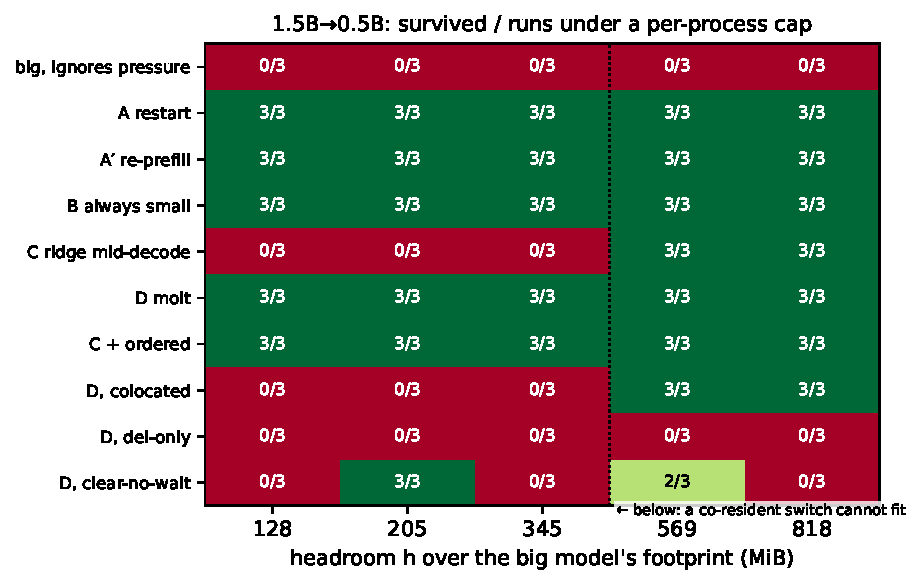
\includegraphics[width=\linewidth]{../figures/paper/memory_survival.pdf}
\caption{Experiment M. Survival rate against headroom $h$ over the big model's own footprint, one process per run under the jetsam emulator. The dotted line marks the headroom a co-resident switch needs (receiver weights $+$ mapper $+$ margin).}
\label{fig:survival}
\end{figure}

\begin{table}[t]\centering\small
\caption{Memory schedules. All of them compute the same transfer; they differ only in what is resident when.}
\label{tab:schedules}
\begin{tabular}{lll}\toprule
schedule & order & resident at peak \\\midrule
colocated & load receiver, map, drop sender & sender $+$ receiver $+$ mapper \\
del-only & drop sender refs, map, load receiver & sender (cached by MLX) $+$ receiver \\
clear-no-wait & drop, \texttt{clear\_cache()}, load at once & depends on reclaim timing \\
ordered & drop, sync, clear, \emph{wait}, map, drop mapper, load & $\max(\text{sender}, \text{KV}+\text{mapper}, \text{receiver})$ \\
\bottomrule\end{tabular}
\end{table}

\section{Where the hypothesis fails, stated plainly}\label{sec:failures}
\pending{written once all measurements are in.}


\section{Limitations}\label{sec:limits}
\begin{itemize}
\item \textbf{No iPhone results yet.}
Every number in this draft comes from an M2 Mac with a jetsam \emph{emulator}.
The device protocol is written and its platform core is self-tested on macOS (\texttt{ios/}).
It covers the Memory Budget Test that reproduces real kills, Instruments traces, and at least three device generations.
The app itself has not been compiled or run, because the build machine's Xcode license is not accepted and no device is attached.
The simulator is not used: it enforces no per-app limit.
Real limits, the \texttt{increased-memory-limit} entitlement, and iOS's own reclaim timing could all move the band of \cref{sec:results-memory}.
\item \textbf{A shared, overloaded machine.}
Other users' processes kept swap nearly full throughout.
Footprint, survival and quality are unaffected.
Times and GPU energy are inflated and noisy, and are reported with the machine's load average.
\item \textbf{Energy is partial.}
CPU energy is per process.
GPU energy is system-wide minus an idle baseline.
DRAM energy is missing.
A \texttt{powermetrics} cross-check is pending.
\item \textbf{Human ratings are pending.}
The seam is measured only with a model judge, which is the pair's own large model.
\item \textbf{Scope.} One model family (Qwen2.5), 4-bit weights, greedy decoding, English text.
\end{itemize}

\section{Conclusion}\label{sec:conclusion}
We moved a generation from a larger to a smaller model mid-decode, triggered by the app's headroom, without ever holding both.
Against a faithful reproduction of the closed-form KV map of~\citep{heo2026crossmodel}, the measurements give one result that holds and two that do not.
\begin{itemize}
\item \textbf{Holds.} The memory order decides survival. Loading the receiver before releasing the sender, as a prefill hand-off does, is killed whenever headroom is below the receiver plus mapper. Releasing first survives.
\item \textbf{Does not hold.} Mapping the cache did not carry the prompt's content into the small model, with or without our anchors.
\item \textbf{Does not hold.} Re-reading the transcript was better on every quality measure, and also faster at the context lengths we ran.
\end{itemize}
For an on-device app facing a per-process limit mid-answer, our data recommend a release-first re-prefill, not KV transfer.
Device measurements on iPhones (\cref{sec:limits}) are the next step, because iOS's own limits and reclaim behaviour could move the band.



\bibliographystyle{plainnat}
\bibliography{refs}

\appendix
\section{What freeing a model costs on MLX}\label{app:mlx}
All three facts below are measured by \texttt{mlx/molt\_mlx/footprint.py::selftest} on every run of the test suite.
\begin{enumerate}
\item A 256\,MiB MLX array adds \res{mlx.alloc_fp}\,MiB to phys\_footprint, while total RSS is \res{mlx.alloc_rss}\,MiB.
\item After \texttt{del} the footprint is unchanged (+\res{mlx.after_del}\,MiB).
\texttt{mx.clear\_cache()} immediately after \texttt{del}, followed by a 300\,ms sleep, freed the buffer in only \res{mlx.clear_alone_freed} of \res{mlx.release_runs} runs; in the others the footprint stayed up by as much as +\res{mlx.after_clear_max}\,MiB.
Whether it frees depends on whether the GPU has finished with the buffer, so it is not something to rely on.
\item \texttt{mx.synchronize()}, then \texttt{clear\_cache()}, then polling returned the memory every time, with a median of \res{mlx.release_ms}\,ms (range \res{mlx.release_ms_min}--\res{mlx.release_ms_max}\,ms).
\end{enumerate}
The peak-footprint test (\texttt{mlx/tests/test\_peak\_footprint.py}) runs each schedule in its own process under a cap of (source-resident footprint $+$ 40\,MiB).
The models are a synthetic \res{peak.src_mib}\,MiB source and a \res{peak.dst_mib}\,MiB destination, so the cap is below source plus destination.
Ordered peaks at \res{peak.ordered_mib}\,MiB under a \res{peak.cap_mib}\,MiB cap; colocated and del-only are killed in \texttt{load\_dst}.
clear-no-wait survived \res{peak.cnw_survived} of 3 runs at this size, so it is \emph{not} shown to fail there; the full-size result is in \cref{sec:results-memory}.

\section{Energy without root}\label{app:energy}
\texttt{ri\_energy\_nj} counts CPU energy only: a busy MLX matmul loop reads \res{energy.gpu_loop_proc_w}\,W in it.
IOReport's ``GPU Energy'' channel reads \res{energy.gpu_loop_gpu_w}\,W for the same loop, with no root required.
Energy is reported as these two named parts and never summed silently.
DRAM energy is unavailable without \texttt{powermetrics}; \texttt{bench/powermetrics.sh} is the root cross-check.

\section{Reproducing every number}\label{app:repro}
{\small\begin{verbatim}
python -m pytest mlx/tests --import-mode=importlib  # selftests + peak test
python -m bench.facts                     # MLX freeing + energy facts
python -m bench.fit_mappers --pair 1.5b-0.5b   # fit, sweep, select
python -m bench.intrinsic   --pair 1.5b-0.5b   # experiment I
python -m bench.run_memory  --pair 1.5b-0.5b   # experiment M
python -m bench.run_quality --pair 1.5b-0.5b   # experiment Q
python -m bench.score       --pair 1.5b-0.5b   # judge scores
python -m bench.analyze                   # bench/results/summary.json
python figures/make_paper_figures.py      # figures + this paper's macros
python -m bench.make_results_md           # RESULTS.md
cd ios && swift run MoltCoreSelfTest      # Swift core
\end{verbatim}}
\noindent \texttt{python -m bench.run\_all} runs the middle block for both pairs, resumably.
Figures and every number in the text are produced from \texttt{bench/results}; none is typed by hand.

\end{document}
